\documentclass[mathserif,xcolor=dvipsnames]{beamer}

\usepackage{pset}

\usepackage{graphicx}
\usepackage{amssymb}
\usepackage{mathtools}

\usetheme{Madrid}
\usecolortheme[named=RawSienna]{structure} 
\useoutertheme{umbcfootline} 
%\usetheme[height=7mm]{Rochester} 
\setbeamertemplate{items}[ball] 
\setbeamertemplate{blocks}[rounded][shadow=true] 
\setbeamertemplate{navigation symbols}{} 


\renewcommand*{\Z}{\mathbbm{Z}}
\renewcommand*{\R}{\mathbbm{R}}
\renewcommand*{\C}{\mathbbm{C}}
\newcommand*{\B}{\mathcal B}
\DeclareMathOperator*{\argmax}{arg max}

\title[The Geometry of DBNs]{The (Real) Geometry of \\the Restricted Boltzmann Machine}
\author{Aaron Pribadi}
\institute[HMC]{Harvey Mudd College}
\date{November 8, 2011}

\begin{document}

\begin{frame}[plain]
    \maketitle
\end{frame}


\begin{frame}{The Probability Simplex}
    Probability distribution over $[N] = \{1,2,\ldots, N\}$:
    \[
        p(k) = x_k,
        \qquad
        \text{where }
        \sum_k x_k = 1,
        \;
        x_k > 0.
    \]

    The $(N-1)$-dimensional \textbf{probability simplex} is the space of
    distributions:
    \[
        \Delta_{N-1} = \cdil*{(x_1, \ldots, x_N) 
        \;\Bigl\vert\;
        \sum_k x_k = 1,\; x_k \ge 0}
        \subset
        \R^N.
    \]
\end{frame}

\begin{frame}
    \linespace
    \linespace
    \begin{center}
    \scalebox{0.5}{ 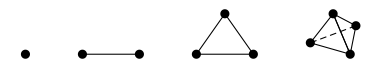
\includegraphics[scale=1]{simplices.png} }
    \end{center}
\end{frame}

\begin{frame}{Binary Independence Model}
    Consider distributions over the states
    \[
        v = (v_1, \ldots, v_n) \in \{0,1\}^n
    \]
    of the form
    \[
        p(v) = \prod_{i=1}^n\; \lambda_i^{v_i} (1 - \lambda_i)^{1-v_i}
        \qquad
        \text{with }\lambda_i \in (0,1).
    \]
    The \textbf{binary independence model} is the space 
    \[
        B \subset \Delta_{N-1}
        \qquad\text{where $N = 2^n$},
    \]
    of all such distributions, and is an $n$-dimensional hypersurface.
\end{frame}

\begin{frame}{Restricted Boltzmann Machine}
    The \textbf{restricted Boltzmann machine} is a model over $n$ visible nodes
    and $k$ hidden nodes, all binary.
    \begin{center}
    \scalebox{0.7}{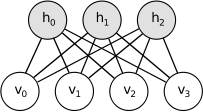
\includegraphics{rbm.png}}
    \end{center}
    \vspace{-0.3cm}
    The distribution over the space $\{0,1\}^n$ of visible states is
    \[
        p(v) = \frac 1 Z \sum_{h \in \{0,1\}^k}
        \exp\pdil*{
            \sum_{ij} w_{ij} v_i h_i + \sum_i b_i v_i + \sum_j c_j h_j
        }
    \]
    where $Z$ is a normalizing constant, the $w_{ij}$ are weights on the edges,
    and $b_i$ and $c_j$ are biases on the visible and hidden nodes
\end{frame}

\begin{frame}{Restricted Boltzmann Machine}
    Proposition (Cueto, Morton, Sturmfels):
    
    \linespace
    \textit{Let $M_n^k \subset \Delta_{N-1}$ be the RBM model
    with $n$ visible and $k$ hidden nodes.  Then the model factors as
    \[
        M_n^k = (M_n^1)^{[k]}
    \]
    where the right side is the $k$-th Hadamard power of the model with one
    hidden node.}
\end{frame}

\begin{frame}{One Hidden Node}
    The model with one hidden node, $M_n^1$, contains distributions of the form
    \[
        p(v) = \eta \pdil*{\prod_i \lambda_i^{v_i} (1 - \lambda_i)^{1 - v_i}}
        + (1 - \eta) \pdil*{\prod_i \mu_i^{v_i} (1 - \mu_i)^{1 - v_i}}
    \]
    i.e. is the mixture of two binary independence models.

    \linespace
    (Here, $\lambda_i, \mu_i \in (0,1)$ and $\eta \in [0,1]$.)
\end{frame}

\begin{frame}{Hadamard Product}
    The Hadamard product $p * q$ of two (strictly positive) distributions is 
    \[
        (p*q)(v) = \frac{p(v)q(v)}{\sum_w p(w) q(w)}
    \]
    where the normalizing constant in the denominator is a sum over all states.

    \linespace
    (It is essentially coordinate-wise multiplication.)

    \linespace
    By a Hadamard power, we mean the space
    \[
        M^{[k]} = \cdil[\big]{ m_1 * \cdots * m_k \mid m_i \in M }.
    \]
\end{frame}

\begin{frame}{Nested Models}
    It is easy to show that the models nest
    \[
        M_n^0 \subset M_n^1 \subset 
        \cdots \subset M_n^k \subset 
        \cdots \subset \Delta_{N-1}.
    \]
    Question: What does this nesting look like?
\end{frame}

\begin{frame}{Dimension Counting}
    Conjecture (Cueto, Morton, Sturmfels):
    
    \linespace
    \textit{The restricted Boltzmann machine has the expected dimension,
    i.e. $M_n^k$ is a semialgebraic set of dimension $\min\,\{nk + n + k, 2^n -
    1\}$ in $\Delta_{2^n - 1}$.
    }

    \linespace
    This result was proved in their paper for almost all cases.
\end{frame}

\begin{frame}{Universal Approximation}
    Theorem (Ay, Montufar):

    \linespace
    \textit{With $k = 2^{n-1} -1$, the model $M_n^k$ is dense in
    $\Delta_{2^n-1}$.}

    \linespace
    This result was proved by construction, and is likely not sharp.
\end{frame}


\begin{frame}{Writing Old Things in New Ways}
    From the proposition of Cueto et al., it is not hard to show that every
    distribution in the RBM model is of the form
    \[
        \sum_{h \in \{0,1\}^k}
        \pdil*{
            \prod_i \eta_i^{h_i} (1 - \eta_i)^{1 - h_i}
        } b_h
    \]
    where
    \[
        b_h = a_1^{h_1} * a_2^{h_2} * \cdots * a_k^{h_k}
    \]
    and the $a_i^{h_i}$ are from the binary independence model.

    \linespace
    That is, the RBM is a mixture model of binary independence models, where
    both weights and models are constrained.
\end{frame}

\begin{frame}{Writing Old Things in New Ways}
    Then,
    \[
        M_n^k = \cdil[\Big]{
            \eta(m * f) + (1 - \eta)(m * g)
            \;\big\vert\;
            m \in M_n^{k-1},\;
            f,g \in B,\;
            \eta \in [0,1]
        }.
    \]

    \linespace
    My current approach is to attempt to bound how much the model expands using
    some appropriate notion of distance.

    \linespace
    An examination reveals that we have extra `degrees of freedom'. It would be
    nice to work with distributions `modulo the binary independence model'.
\end{frame}

\begin{frame}{Some Groups}
    The space $\Delta_{N-1}$ of (strictly positive) distributions is an abelian
    group under the Hadamard product.  Indeed
    \begin{align*}
        e &= \pdil*{ \tfrac 1 N, \ldots, \tfrac 1 N }\\
        \inv p &= \tfrac 1 Z \pdil*{ \tfrac{1}{p_1}, \ldots, \tfrac{1}{p_N} }
        & Z = \sum_i \tfrac{1}{p_i}.
    \end{align*}

    \linespace
    There is in fact a group isomorphism
    \[
        (\Delta_{N-1}, *) \cong (\R^N, +) / \{(x, \ldots, x) \mid x \in \R\}
    \]
    given by
    \[
        p = (p_1, \ldots, p_N) \longleftrightarrow (\log p_1, \ldots, \log p_N).
    \]
\end{frame}

\begin{frame}{Some Groups}
    The binary independence model $B \subset \Delta_{N-1}$ is a subgroup of
    $(\Delta_{N-1}, *)$.

    \linespace
    The quotient $\Delta_{N-1} / B$ is a good space with which to work.
    \begin{itemize}
        \item $M_n^k$ is invariant under the action of $B$.
        \item Under the quotient projection, $M_n^0$ goes to $[0]$.
        \item Modulo $B$, every $p \in M_n^k$ is determined by a sequence
        \[
            0 = p_0 \mapsto p_1 \mapsto \cdots \mapsto p_k = p
        \]
        where each transition is determined by a pair $(f, \eta)$, with $f \in
        B$ and $\eta \in [0,1]$.
    \end{itemize}
\end{frame}

\begin{frame}{Where To?}
    Questions:
    \begin{itemize}
        \item What is a parametrization of $\Delta_{N-1} / B$?
        \item Do ways to measure distances between distributions (e.g.
        Kullback-Leibler divergence, total variation distance, Euclidean
        distance) project well to $\Delta_{N-1} / B$?
        \item Can this help with the original goal, i.e. what is the minimal $k$
        such that $M_n^k$ is dense in $\Delta_{N-1}$?
    \end{itemize}

    Things to look at:
    \begin{itemize}
        \item There is a natural symmetry group $S_n \ltimes (S_2)^n$.
        \item Algorithms in real algebraic geometry.
    \end{itemize}
\end{frame}

\begin{frame}{References}
\begin{thebibliography}{100}
    \bibitem{RBM2} Ay, Montufar.  ``Refinements of Universal Approximation
    Results for Deep Belief Networks and Restricted Boltzmann Machines''.
    2011.
    \bibitem{RBM} Cueto, Morton, Sturmfels. ``Geometry of the Restricted
    Boltzmann Machine''.  2009.
\end{thebibliography}
\end{frame}

\end{document}
